%!TEX root = ../report.tex

% 
% Architecture
% 

\section{Architecture}

%introduction

A refactoring tool that would suit an unexperienced programmer who is learning how to program is needed. 
Racket is a dynamic language that is known of being used as an introductory programming course in schools around the world. 
Racket also has an IDE, DrRacket that is a pedagogic environment \cite{drscheme_pegadogy} and it also supports development and extension of other programming languages \cite{tobin2011languages} and recently it has an implementation of python \cite{ramos2014implementation}.
Besides that, DrRacket only has one refactoring operation, that is the rename.
That will motivate the unexperienced programmers to start using tool assisted refactoring operations and DrRacket seams to be the ideal candidate to have that refactoring tool.


%use cases: To validate the architecture.
\subsection{Refactoring Operations Desired}
%Das operacoes para a refactoring tool vamos falar particularmente destas, ou por exemplo destas.
There are some refactoring operations that were already chosen because of theirs importance.
%introduce the validate cases xD

% rename improved
\subsubsection{Rename}
%this is a refactoring for racket
The rename is the most used refactoring operation and it is indispensable to any refactoring tool.
Nevertheless, DrRacket already has a rename operation, however the rename is not suit for renaming imported functions.
When renaming a imported function the original rename of DrRacket renamed the name all the functions imported from the same file and the name of the file. However this is not the correct action, DrRacket should only rename the function with the selected name.
This situation happens when using functions exported from another file or library it is necessary to require them, in other words to import.
After that, the user can call the methods exported like they were defined in the file.
However those methods could have name collision or change it for a more adequate name. To do that the user would do a rename.


% extract-function
\subsubsection{Extract-function}

Extract functions is a simple and very useful refactoring, and it is shown previously in this document that is one of the most used refactoring operations.

Extract-function is an important refactoring for unexperienced users since those users tend to create a big function that does all the work.

By having a mean to restructure the code, unexperienced programmers will be able to create programs with better quality.




\subsubsection{Move expression}

Move expression is also one of the most used refactoring operations.
This operation allows the user to move safely the expressions to the new location.



% add-prefix
\subsubsection{Add-prefix}
%this is a refactoring for racket only!
This is 
A programmer when using some functions from a library and then realizes that needs another library. when importing that library conflicts occur.
both libraries have function with the same name. The solution add a prefix for one of the requires.
That is really annoying because the user has to remember and change one by one all functions invocations.

The Add Prefix refactoring does all that for the user.

This is also useful when the name of the functions are similar, adding a prefix make it easier to distinguish between libraries.





\subsection{Structure}
%s-exp and def-uses-relationships

%An image will be awesome here
The architecture of the refactoring tool will consist in an AST and in the def-use-relations of the program.
The information gathered in the AST and in the def-use-relations with some preconditions is enough to ensure the correctness of the refactoring operations.
The AST in the Racket programing language is composed of s-expressions. Because a program is a list of s-expressions.
DrRacket provides the def-use-relations which is an important help to do the refactoring operations. The def-use-relations are visual represented as arrows in the DrRacket.

\begin{figure}[htbp]
	\centering
	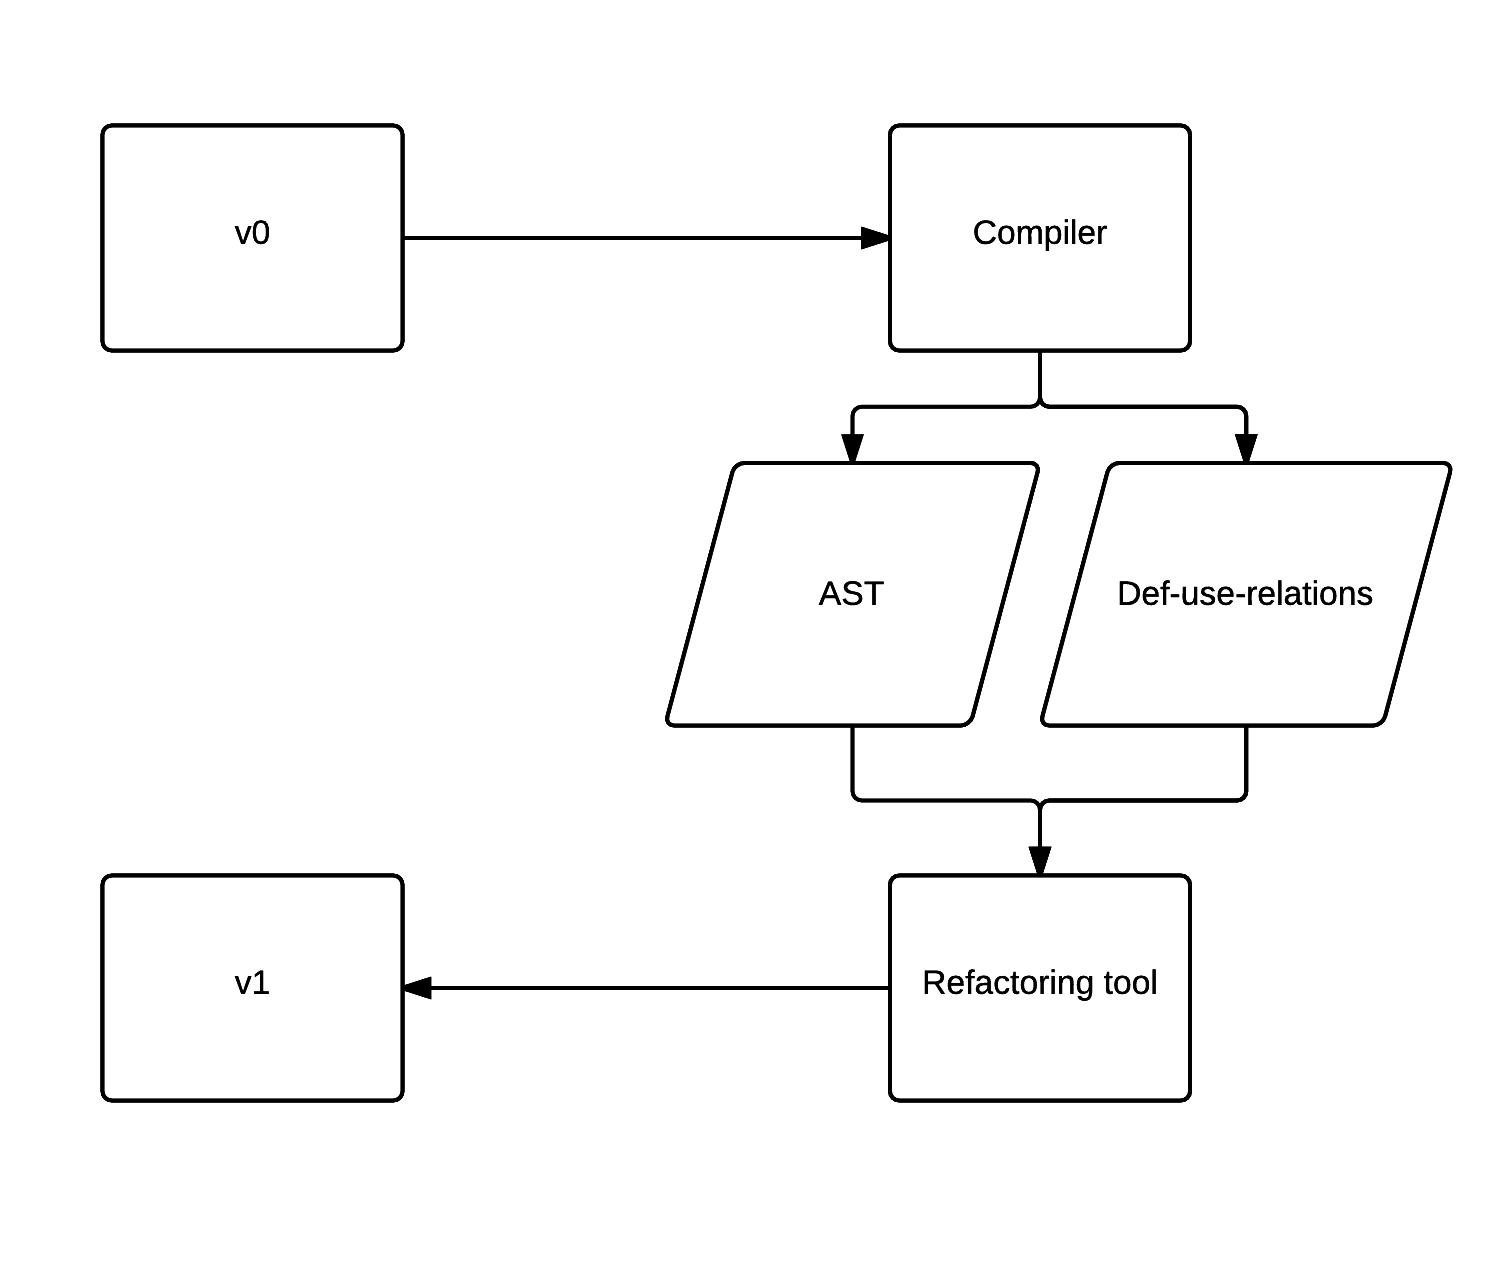
\includegraphics[width=0.95\textwidth]{img/arquitectura.png}
	\caption{Solution's architecture}
	\label{fig:label}
\end{figure}

\subsection{Validation}
%In order to evaluate it was implemented a prototype in DrRacket.
In order to validate this architecture some refactoring operations were implemented. 
This allows to validate the architecture and have more trust in this architecture.
To do that it was only validated the refactoring operations that only used the def-use-relations.

\subsubsection{Extract-method}
\subsubsection{Imported renames}
\subsubsection{Add-prefix}

